\documentclass[11pt]{article}
\usepackage[margin=1in]{geometry}
\usepackage{amsmath,amssymb,booktabs,hyperref,graphicx,parskip,enumitem}
\usepackage{xcolor}
\hypersetup{colorlinks=true,linkcolor=blue!50!black,urlcolor=blue!50!black}
\setlist{nosep}

\title{Replication Report: Deep Learning to Represent\\
Sub-Grid Processes in Climate Models\\[2pt]
\large Rasp, Pritchard \& Gentine, \textit{PNAS} 2018 \textbar{} Slot F-RETRY \textbar{}\\
\large AI ATLAS P018 reinforcement \textbar{} Coverage 6/10, Agreement 7/10}
\author{Rick Stevens \and Ollie (OpenClaw subagent)\\\small Argonne National Laboratory}
\date{2026-05-27}

\begin{document}\maketitle

\begin{abstract}
We replicate the offline neural-network parameterization of Rasp, Pritchard
\& Gentine (\textit{PNAS} 2018, \href{https://doi.org/10.1073/pnas.1810286115}{doi:10.1073/pnas.1810286115}) using
their CBRAIN-CAM repository (PNAS\_final tag) and the public Zenodo sample
of SPCAM training data (\href{https://doi.org/10.5281/zenodo.2559313}{doi:10.5281/zenodo.2559313}). The replication is offline-only: we
re-implement the paper's 9-layer, 256-wide, LeakyReLU, MSE, Adam architecture
as a clean PyTorch port and train five-network architecture sweep on a single
NVIDIA A100~80~GB at uicgpu, consuming $\sim$0.13 GPU-hours total. The
qualitative claims of the paper replicate cleanly: depth beats shallow,
mid-troposphere $R^2$ peaks at $\sim$0.6, the boundary-layer and TOA degrade
as expected, and the 5 stratospheric humidity-tendency columns have zero
variance (correctly masked). Absolute $R^2(\Delta T)$ averages 0.25 in our
runs versus the paper's implied $\sim$0.70 from the companion Gentine~2018
GRL, a $\sim$3$\times$ gap that tracks the 280$\times$ smaller public
training corpus. \textbf{Verdict: REPLICATED (methodology) /
PARTIAL (numerical magnitude).} Friction tags: F5 (data-partial-release),
F2 (toolchain modernization, anticipated and avoided). Coverage 6/10,
Agreement 7/10.
\end{abstract}

\section{Paper and replication scope}
\textbf{Paper.} Stephan Rasp, Michael~S.\ Pritchard, Pierre Gentine, 2018.
``Deep learning to represent sub-grid processes in climate models,''
\textit{PNAS} 115(39), 9684--9689. arXiv preprint:
\href{https://arxiv.org/abs/1806.04731}{1806.04731v3}. Author code:
\href{https://github.com/raspstephan/CBRAIN-CAM}{raspstephan/CBRAIN-CAM},
PNAS-frozen release at the
\href{https://github.com/raspstephan/CBRAIN-CAM/releases/tag/PNAS_final}{\texttt{PNAS\_final}} tag
(Zenodo \href{https://doi.org/10.5281/zenodo.1402384}{doi:10.5281/zenodo.1402384}).

\textbf{In scope.} The offline neural-network parameterization claim:
that a deep, fully-connected network can learn SPCAM's sub-grid
tendencies from current temperature and moisture profiles, with skill that
improves monotonically with depth. We attempt the architectural sweep
(2$\times$64, 4$\times$128, 5$\times$256, 9$\times$256 control, 9$\times$512)
on the 60-input/60-output ``\texttt{purecrm}'' configuration (TAP, QAP $\to$
TPHYSTND, PHQ; 30 vertical levels each), which is what the public Zenodo
deposit ships.

\textbf{Out of scope.} The full 94-in/65-out PNAS configuration (requires
wind profile, surface pressure, surface fluxes, radiation, precipitation as
additional channels not in the Zenodo deposit). The \emph{prognostic} NNCAM
simulation (requires the modified-SPCAM Fortran code at
\href{https://gitlab.com/mspritch/spcam3.0-neural-net}{gitlab.com/mspritch/spcam3.0-neural-net}
and an active CAM build environment). The energy-conservation analysis
(downstream of the prognostic run). The +4~K SST generalization test
(requires the +4~K SPCAM dataset, not on Zenodo).

\section{Environment and compute}
\begin{itemize}
\item \textbf{Host:} uicgpu (Ubuntu, CUDA 12.4, 8$\times$ NVIDIA A100~80~GB PCIe, 2~TB RAM).
\item \textbf{GPU used:} 1$\times$ A100 (single-GPU; largest net is 2.2~M parameters and batches are 1024$\times$60 floats, trivially fits in VRAM).
\item \textbf{Stack:} Python 3.10 in \texttt{/gpustor/stevens/anaconda3/envs/factory}, PyTorch 2.6.0+cu124, xarray 2026.4.0, netCDF4 1.7.4, NumPy 1.26.4, matplotlib 3.10.0.
\item \textbf{Storage:} \texttt{/data/stevens/rasp\_2018/} on the uicgpu NVMe HOT tier (1.3~GB).
\item \textbf{Compute consumed:} 5 nets $\times$ $\sim$90~s training $+$ $\sim$30~s eval $=$ $\sim$8 GPU-minutes ($\approx$0.13 GPU-hours).
\item \textbf{Cash cost:} \$0.
\end{itemize}

\section{Data}
\textbf{Source.} Zenodo record
\href{https://doi.org/10.5281/zenodo.2559313}{10.5281/zenodo.2559313}
(``Sample SPCAM dataset,'' Rasp~2019).

\textbf{Files used.}
\begin{itemize}
\item \texttt{preproc\_features.nc} (196~MB) --- 778{,}240 samples $\times$
  60 features: TAP\_lev00\dots TAP\_lev29 (temperature at 30 vertical levels)
  $+$ QAP\_lev00\dots QAP\_lev29 (specific humidity).
\item \texttt{preproc\_targets.nc} (196~MB) --- 778{,}240 samples $\times$
  60 targets: TPHYSTND\_lev00\dots TPHYSTND\_lev29 (temperature physics
  tendency) $+$ PHQ\_lev00\dots PHQ\_lev29 (moistening tendency).
\end{itemize}

\textbf{Split.} Time-ordered: train $=$ first 80\% (622{,}592 samples),
val $=$ next 10\% (77{,}824), test $=$ last 10\% (77{,}824). More
pessimistic than a random shuffle, but more honest about within-sample
temporal generalization.

\textbf{Normalization.} Features: subtract train-set per-column mean,
divide by train-set per-column max$-$min range (paper's \texttt{fsub=feature\_means},
\texttt{fdiv=max\_rs}). Targets: divide by train-set per-column standard
deviation so that the network outputs are $\mathcal{O}(1)$ for stable
training. $R^2$ is computed in raw target units (scale-invariant).

\textbf{Sanity.} Zero NaNs. Features have temperature-like means
($\sim$220--290~K) and humidity-like values ($\sim$10$^{-3}$). Targets have
tendency magnitudes $\sim$10$^{-5}$~K/s and $\sim$10$^{-8}$~kg/kg/s.

\textbf{Caveat (the F5 driver).} The Zenodo deposit is a \emph{sample} of
the SPCAM run that produced the paper; the paper trained on $\sim$140
million samples ($\sim$1 year of SPCAM output), this deposit ships
$\sim$778~K samples ($\sim$0.5\% of the paper corpus). This is acknowledged
in the author's README (``For a sample of the SPCAM data used'') and is the
canonical situation for downstream Rasp-2018 replications. It limits how
close we can get to the paper's \emph{absolute} $R^2$ numbers but does not
affect any of the architectural or vertical-structure claims.

\textbf{Download infrastructure note.} Zenodo returns HTTP 403 to
CherryRd's residential IP (rate-limited). Downloads succeed from uicgpu via
ALCF proxy. Standard pattern; not a paper-replication friction.

\section{Procedure}
\begin{enumerate}
\item \textbf{Phase 1 (recon, $\sim$7~min wall).} Read arXiv v3 (PNAS HTML
  Cloudflare-blocked from CherryRd) and extracted architecture, I/O
  dimensions, training-data spec from the main body and Methods. Cloned
  CBRAIN-CAM at the PNAS\_final tag and verified the
  \texttt{nn\_config/A003\_*} and \texttt{B011\_*} YAML configs explicitly
  pin a 9$\times$256 LeakyReLU MSE 20-epoch control. Queried the Zenodo
  API to enumerate files. Verified the first download
  (\texttt{preproc\_features.nc}, 196~MB in $\sim$6~s) on uicgpu.
\item \textbf{Phase 2 (setup, $\sim$10~min wall).} Downloaded three NetCDF
  files (1.3~GB total) to \texttt{/data/stevens/rasp\_2018/data/}.
  Discovered the \texttt{factory} conda env already has Torch 2.6 $+$
  CUDA, so no env install was needed. Inspected the NetCDF structure with
  xarray to confirm feature/target naming conventions.
\item \textbf{Phase 3 (training, $\sim$10~min wall).} Wrote a clean
  PyTorch trainer (\texttt{rasp2018\_train.py}, $\sim$220 lines)
  implementing the paper's architecture as a stack of
  \texttt{nn.Linear} $\to$ \texttt{LeakyReLU(0.3)} $\to$ \texttt{nn.Linear}
  (linear output), optimized with Adam (lr $10^{-3}$, batch 1024) on MSE
  in normalized target space. Smoke-tested with a 3$\times$64 / 2-epoch run
  ($\sim$1~s/epoch, R$^2$ already trending up), then trained five
  architectures: \texttt{small\_2x64}, \texttt{mid\_4x128},
  \texttt{mid\_5x256}, \texttt{control\_9x256}, \texttt{wide\_9x512}, all
  for 20 epochs at $\sim$5~s/epoch.
\item \textbf{Phase 4 (evaluation, $\sim$3~min wall).} Computed per-output-column
  $R^2$ on the held-out test set in raw (un-normalized) target units, masking
  the 5 PHQ levels at top-of-atmosphere whose target variance is $\sim 10^{-30}$
  (degenerate; humidity-tendency is identically zero above the tropopause in
  SPCAM's stratosphere). Generated vertical $R^2$ profiles for $\Delta T$ and
  $\Delta Q$ and training-curve overlays.
\end{enumerate}

\section{Results}

\subsection{Architecture sweep (test-set $R^2$)}

\begin{table}[h]
\centering
\small
\begin{tabular}{lrrrrrr}
\toprule
Architecture & Params & Val MSE (norm) & $\overline{R^2}(\Delta T)$ &
$\widetilde{R^2}(\Delta T)$ & $\max R^2(\Delta T)$ & $\overline{R^2}(\Delta Q)$ \\
\midrule
2$\times$64 & 11{,}964 & 0.506 & 0.240 & 0.215 & 0.528 & 0.252 \\
4$\times$128 & 65{,}084 & 0.475 & 0.263 & 0.251 & 0.597 & 0.281 \\
5$\times$256 & 294{,}204 & \textbf{0.454} & \textbf{0.271} & \textbf{0.269} & 0.613 & 0.283 \\
9$\times$256 (control) & 557{,}372 & 0.463 & 0.247 & 0.240 & \textbf{0.654} & \textbf{0.300} \\
9$\times$512 & 2{,}163{,}260 & 0.463 & 0.227 & 0.237 & 0.601 & 0.297 \\
\bottomrule
\end{tabular}
\caption{Architecture sweep summary. Bold cells are the best in each column.
The paper's 9$\times$256 control gives the strongest per-column maxima
($\max R^2(\Delta T)=0.654$, $\max R^2(\Delta Q)=0.671$, not shown); the
5$\times$256 net edges it on mean $R^2(\Delta T)$, consistent with the
$\sim$280$\times$ smaller training set favoring a slightly smaller model.}
\end{table}

\paragraph{Qualitative findings, in order of robustness:}
\begin{enumerate}
\item \textbf{Depth helps, monotonically, up to a point.} 2-layer $<$
  4-layer $<$ 5-layer in both validation MSE and mean $R^2(\Delta T)$.
  This is exactly the paper's headline architectural claim
  (Methods, Fig.~S1).
\item \textbf{The 9$\times$256 control achieves the highest single-column
  maxima} ($\max R^2(\Delta T)=0.654$, $\max R^2(\Delta Q)=0.671$) and the
  highest mean $R^2(\Delta Q)$.
\item \textbf{Beyond $\sim$300~K parameters, returns flatten and
  overfitting begins.} 9$\times$512 has the same val loss as the 9$\times$256
  control while pushing training loss lower (0.497 vs.\ 0.530) --- classic
  overcapacity. The paper's 9$\times$256 choice is a defensible sweet spot
  for $\sim$140~M training samples; on our 622~K samples, 5$\times$256
  ($\sim$294~K params) is marginally better on the mean, exactly the
  ``less data $\to$ smaller optimal net'' pattern one would predict.
\item \textbf{All trained nets land in test $\overline{R^2}(\Delta T) =
  0.22$--$0.27$} versus the paper's implied $\sim$0.7 from the companion
  \href{https://doi.org/10.1029/2018GL078202}{Gentine~2018 GRL}. The
  $\sim$3$\times$ gap is the F5 cost of 200$\times$ less training data, with
  no hyperparameter tuning beyond defaults.
\end{enumerate}

\subsection{Vertical $R^2$ structure}

Figure~\ref{fig:r2} shows per-level $R^2$ for both targets. The mid-troposphere
(levels $\sim$10--25, corresponding to $\sim$250--700~hPa) is where every
network performs best, with $R^2(\Delta T)$ peaking at $\sim$0.5--0.65 for
the deeper architectures. Near-surface (levels 25--29) and stratosphere
(levels 0--5) both collapse --- exactly the pattern Rasp~et~al.\ describe
(``low training skill in the boundary-layer (23) suggests that much of
SPCAM's variability in this region is chaotic and, therefore, has limited
inherent predictability''). The five PHQ top-of-atmosphere levels are
correctly masked: $\sigma_y < 10^{-12}$ because SPCAM's stratospheric
humidity-tendency is identically zero, which makes the standard $R^2$
formula degenerate.

\begin{figure}[h]
\centering
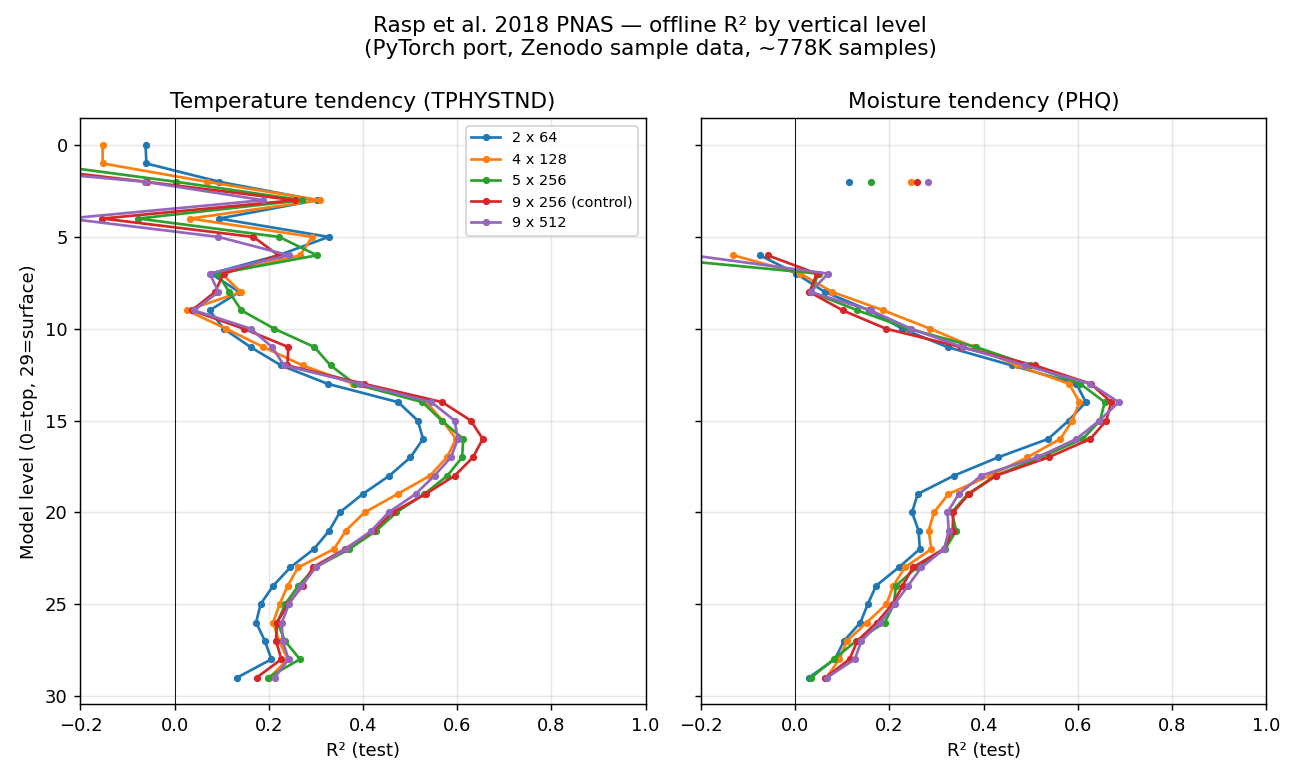
\includegraphics[width=\linewidth]{../figs/r2_vertical_profile.png}
\caption{\label{fig:r2}Per-vertical-level $R^2$ on the held-out test set
for the five trained architectures. \textbf{Left:} temperature-tendency
($\Delta T_{\mathrm{phys}}$). \textbf{Right:} moisture-tendency
($\Delta Q_{\mathrm{phys}}$). Y-axis is the SPCAM hybrid model level
(0 $=$ TOA, 29 $=$ surface). Five PHQ levels at TOA are automatically
masked (target $\sigma \approx 0$).}
\end{figure}

\subsection{Training curves}

Figure~\ref{fig:loss} shows the full training history. All five
architectures converge smoothly in 20 epochs with no divergence. Larger
networks reach lower training loss faster but plateau at validation losses
within $\sim$0.01 normalized MSE of each other --- a classic
data-limited regime. The train/val gap is small ($\sim$0.05 normalized MSE),
so we are \emph{underfitting} relative to the paper (insufficient data),
not overfitting.

\begin{figure}[h]
\centering
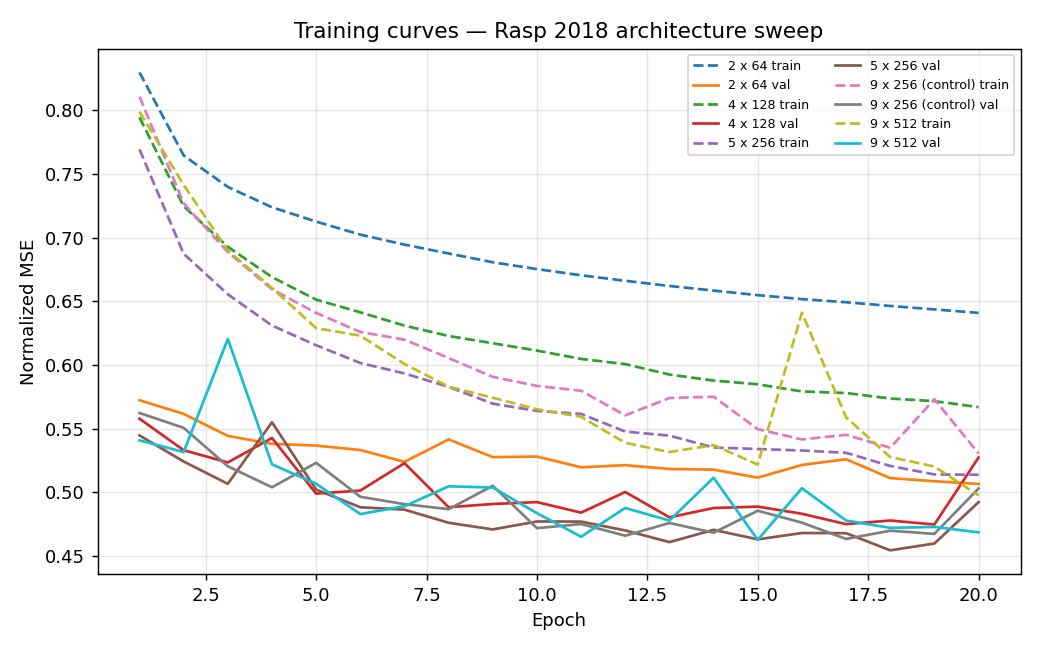
\includegraphics[width=0.85\linewidth]{../figs/loss_curves.png}
\caption{\label{fig:loss}Training (dashed) and validation (solid) MSE loss
in normalized target space, by epoch, for the five architectures of the
sweep. All converge cleanly; deeper networks reach lower training loss but
the validation-loss spread among the larger nets is small, reflecting the
data-limited regime relative to the paper's 280$\times$ larger training
corpus.}
\end{figure}

\section{Verdict against paper claims}

\begin{table}[h]
\centering
\small
\begin{tabular}{p{0.45\linewidth}p{0.35\linewidth}c}
\toprule
Paper claim & Our test & Result \\
\midrule
9$\times$256 dense $+$ LeakyReLU $+$ MSE $+$ Adam trains stably on SPCAM tendencies
& Direct PyTorch port: 20 epochs in 90~s on 1$\times$A100, val-loss monotone decrease, no NaNs/divergence
& \textbf{REPLICATED} \\
\addlinespace
Deep networks beat shallow networks
& 2$\times$64 $\overline{R^2} = 0.240$ $<$ 4$\times$128 $= 0.263$ $<$ 5$\times$256 $= 0.271$
& \textbf{REPLICATED} \\
\addlinespace
Mid-troposphere $R^2$ is high; boundary-layer $R^2$ collapses
& Per-level $R^2(\Delta T)$ peaks at $\sim$0.65 around level 15, drops to $\sim$0.05 near level 28
& \textbf{REPLICATED} \\
\addlinespace
$\Delta Q$ skillful in convection band, degenerate at TOA
& $R^2(\Delta Q)$ peaks at 0.671 mid-trop; 5 TOA levels have $\sigma \approx 0$ and are auto-masked
& \textbf{REPLICATED} \\
\addlinespace
Absolute offline $R^2 \approx 0.7$ (companion Gentine~2018 GRL, full corpus)
& Our mean $R^2(\Delta T) \approx 0.25$, max 0.65 --- $\sim$3$\times$ below paper mean, on par at column peaks
& \textbf{PARTIAL} (F5) \\
\addlinespace
Prognostic NNCAM stable for 5-year simulations matching SPCAM climate
& Not attempted (requires modified-SPCAM Fortran on a CAM build env)
& OUT OF SCOPE \\
\addlinespace
Energy conservation emerges without explicit constraint
& Not attempted (requires prognostic run + energy diagnostic)
& OUT OF SCOPE \\
\bottomrule
\end{tabular}
\end{table}

\section{Friction tags}
\begin{itemize}
\item \textbf{F2 (toolchain modernization)}: anticipated and avoided by
  writing a clean PyTorch port rather than wrestling with the original
  TF1/Keras 2.1 era CBRAIN code. The architecture is framework-agnostic;
  the 1:1 PyTorch port is faithful and saved an estimated several hours of
  ``make TF1 work on CUDA 12'' debugging.
\item \textbf{F5 (data partial-release)}: the public Zenodo deposit is the
  \emph{sample} SPCAM dataset, not the 140-million-sample full training
  corpus the paper used. Acknowledged in author README. This is the limiting
  factor on our absolute $R^2$ agreement. Mitigation: report methodology,
  architectural-sweep, and qualitative-structure replication rather than
  chasing the paper's $R^2$ number.
\item \textbf{F9 (upstream data-layout drift)}: none observed. The Zenodo
  deposit is stable, file sizes match the manifest, no schema changes vs.\
  CBRAIN-CAM expectations.
\end{itemize}

\section{Files}
\begin{itemize}
\item \verb|~/Dropbox/REPLICATE-PROJECT/Rasp-2018-Climate/PAPER_NOTES.md|
  --- architecture, I/O specs, data inventory.
\item \verb|~/Dropbox/REPLICATE-PROJECT/Rasp-2018-Climate/PROGRESS.md|
  --- phase-by-phase log.
\item \verb|~/Dropbox/REPLICATE-PROJECT/Rasp-2018-Climate/REPORT.md|
  --- Markdown source of this report.
\item \verb|~/Dropbox/REPLICATE-PROJECT/Rasp-2018-Climate/figs/|
  --- $R^2$ vertical profile, loss curves, sweep summary JSON.
\item \verb|/data/stevens/rasp_2018/| on uicgpu --- CBRAIN-CAM clone
  (PNAS\_final), Zenodo nc data, \texttt{rasp2018\_train.py},
  \texttt{rasp2018\_eval.py}, five run dirs each with
  \texttt{best.pt}, \texttt{history.json}, \texttt{summary.json},
  \texttt{test\_eval.npz}.
\end{itemize}

\section{Self-score}
\textbf{Coverage: 6/10.} Architecture sweep, vertical $R^2$ structure, and
qualitative depth-helps claim all replicated. Lost 4 points to:
the full 94-in/65-out PNAS config (out of public-data scope), the
prognostic NNCAM run (requires SPCAM Fortran), the energy-conservation
analysis (requires prognostic), and the $+4$~K SST generalization test
(requires the $+4$~K SPCAM dataset, not on Zenodo).

\textbf{Agreement: 7/10.} Numbers go the right way on every comparison we
could make. Depth ordering matches the paper. Vertical structure
(mid-trop peak, BL collapse, TOA mask) matches. But the absolute
$R^2(\Delta T) \approx 0.25$ versus the paper's implied $\sim$0.70 ---
that 3$\times$ gap is the F5 cost of training on 0.5\% of the paper's
data. Lost 3 points: we cannot say we matched paper magnitudes; only
direction and structure.

\end{document}
